%% ------------------------------------------------------------------------- %%
\chapter{Introduction}
\label{cap:introducao}
The study and understanding of human skin color date from many years ago. Being some of the contributors of this field,~\citet{edwards:39} were one of those who tried to precisely analyze the color formation of this particular material. According to them~\citep{edwards:39}, skin is made of a stack of different layers (see Fig.~\ref{fig:human-skin-layers}), each of which reflects a portion of impinging light, after absorbing a certain amount of it by the pigments which lie in the layer. The light which is neither reflected nor absorbed, however, is transmitted through each successive layer to the underlying one, where absorption, reflection, and transmission again take place. The absorption bands of the pigment in each layer are thus "imprinted" on both the reflected and transmitted light from each layer. The total reflected light, consequently, has the absorption characteristics of the pigments in all the layers. This phenomenon gives rise to what we call skin color.


\begin{figure}[!hb]
  \centering
  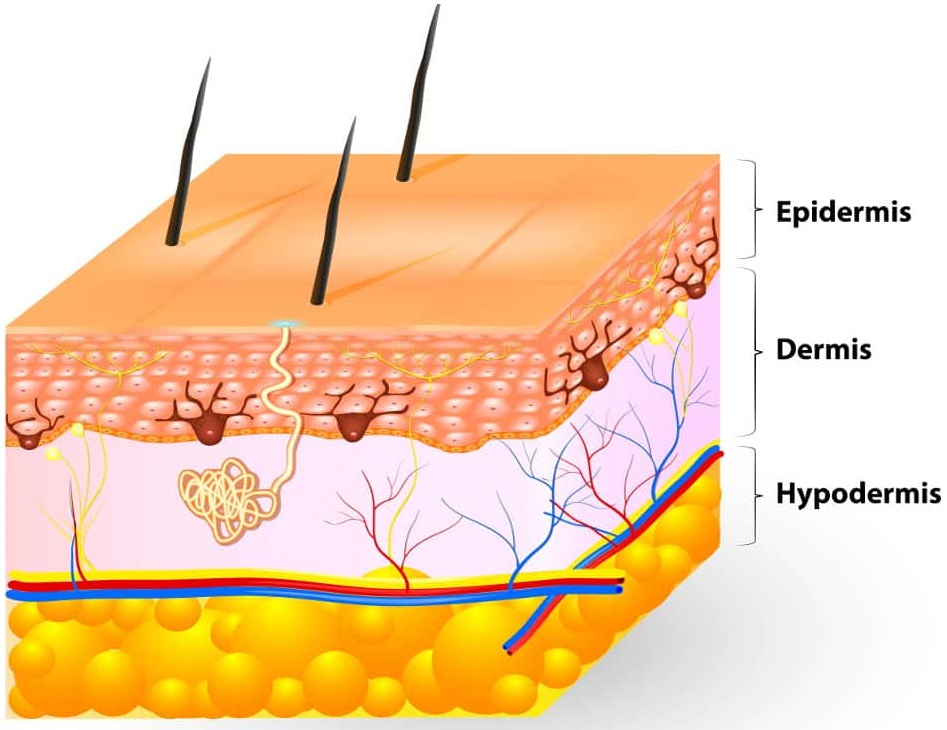
\includegraphics[width=.55\textwidth]{human-skin-layers}
  \caption[The layers of human skin]{The layers of human skin. Source:~\citet{nanette:18}.}
  \label{fig:human-skin-layers}
\end{figure}

\citet{edwards:39} observed yet that other pigments, out of melanin and hemoglobin, also play a role in the origin of skin color, along with an additional optical effect, designated as scattering. The pigments are melanoid -- derivative of melanin --, oxyhemoglobin, and carotene. Furthermore, they stated that variations in the amount of melanin in the epidermis are responsible for the difference in human skin coloration.

Later, \citet{anderson:81} provided an integrated review of the transfer of optical radiation into human skin. They~\citep{anderson:81} noticed that the absorption of Ultra Violet (UV) radiation as well as, to a lesser degree, optical scattering build an optical barrier in the epidermis.

In fact, there is evidence that human skin pigmentation is an adaption for the regulation of penetration of UV radiation into the epidermis. Skin pigmentation of populations has been changed genetically as they moved to parts of the world with different UV radiation levels, a necessary fine-tuning that made it possible for them to tan easily~\citep{jablonski:00}. Tanning is the ability to develop temporary melanin pigmentation in the skin in response to UV radiation and has evolved numerous times in people living under highly seasonal patterns of sunshine~\citep{jablonski:10}.

Therefore, a natural evolution of the skin coloration has been occurred to accommodate the physiological needs of humans as they have dispersed to regions of widely varying annual average UV radiation~\citep{jablonski:10}. On the basis of this observation,~\citet{chaplin:04} built a model for the correlation between the skin reflectance and the seasonal UV radiation levels along with other environmental variables. Based on this model, they~\citep{chaplin:04} could be able to determine the contribution of each variable to skin reflectance. \citet{chaplin:04} combined the data of environmental variables with the UV radiation data recorded by satellite and data on human skin reflectance in a Geographic Information System (GIS). A predicted map of skin color reflectance was produced as a result of the visual and statistical analysis of this system (see Fig.~\ref{fig:skin-ref-map}).


\begin{figure}[!hb]
  \centering
  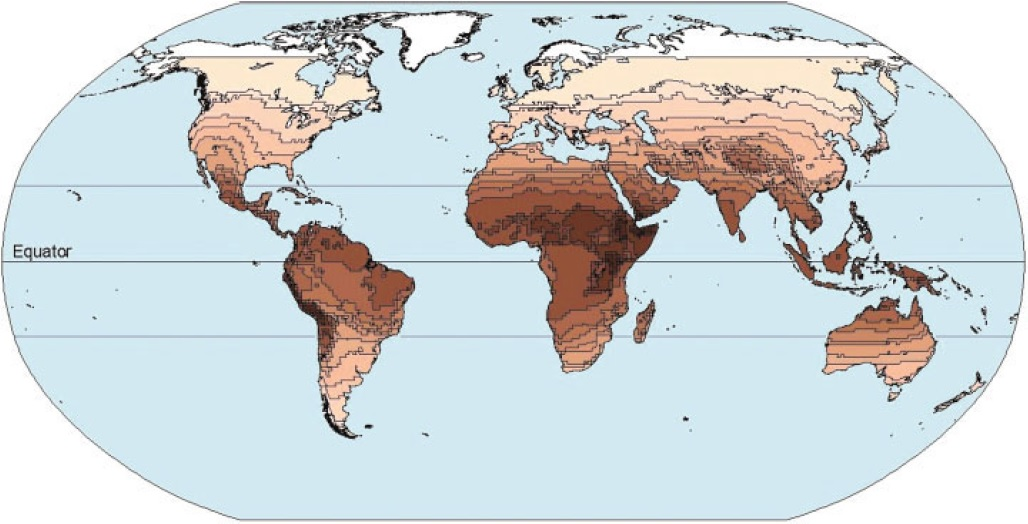
\includegraphics[width=.9\textwidth]{skin-ref-map}
  \caption[Map of skin color reflectance]{Map of skin color reflectance. The map is generalized to reduce the number of polygons. Source:~\citet{chaplin:04}.}
  \label{fig:skin-ref-map}
\end{figure}

We can clearly see darker shades of skin near the Equator and tropics due to exposition to high UV radiation. This is a very singular feature of human skin, once it acts as a sun shield to protect the body from solar UV radiation~\citep{jablonski:04}. The great number of shades of skin shown on the map gives us an idea of how complex can be a system to automatically detect human skin in images, based on color only.

Skin detection can be defined as the process of identifying skin-colored pixels in an image. It plays an important role in a wide range of image processing and computer vision applications such as face detection, pornographic image filtering, gesture analysis, face tracking, video surveillance systems, medical image analysis, and other human-related image processing applications~\citep{kakumanu:07}.

The problem is complex because of the numerous similar materials with human skin tone and texture, and also because of illumination conditions, ethnicity, the large number of shades, sensor capturing singularities, geometric variations, etc. Because it is a primary task in image processing, additional requirements such as real-time processing, robustness, and accuracy are also desirable.

It is worth mentioning that image processing is one of the most important tasks in a computer vision system. Its goal is to create a suitable description -- typically based on shapes, textures, gray levels or color -- with enough information to differentiate the objects in the scene. With this description, useful interpretation can be extracted from the image by means of an automatic computer system that facilitates human perception.

There is no general agreement among authors regarding where image processing stops and computer vision starts. The first, as the title says, processes the image by applying some transformations on it which will produce a more enhanced and readable image. In addition, the input and output of the process are always images. On the other hand, computer vision has the ultimate goal to use computers to emulate human vision, including learning and the ability to make inferences and take actions based on visual inputs. In other words, computer vision is intended to, based on images, obtain more abstract representations~\citep{gonzalez:02}. In general,
computer vision systems benefit from image processing techniques as pre-processing steps to build better applications. Thus, we can see that they definitely are not different fields, but there is an overlapping between them.

This work is intended to explore new methods on human skin detection. We will use techniques from both image processing and computer vision fields. Color space transformation from image processing, for example, as well as human skin segmentation and understanding as part of computer vision. This is a tentative to imitate the human visual system and its capability to recognize others from the same species -- of course, humans use other characteristics to identify other humans like shape, high, gender, and others, but the skin is also part of this recognition system.

One of the powerful features used in this task is definitely skin color, which is a strong attribute and it is used in most algorithms for skin detection. It is normally used along with other features such as shape, texture, and geometry, or even as a preliminary step to classify regions of interest in an image.

The human skin color pixels have a restricted range of hues and are not deeply saturated since the appearance of skin is formed by a combination of blood (red) and melanin (brown, yellow), which leads the human skin color to be clustered within a small area in the color space~\citep{fleck:96}.

Color has the ability of functioning as a descriptor that often simplifies the identification and extraction of an object in a scene. Moreover, the ability of humans to discern thousands of tonalities and intensities compared to only a few dozen levels of gray put the color as a strong candidate feature in computer vision and image processing applications~\citep{gonzalez:02}.

In general, the colors are represented by their brightness, hue, and saturation, which are usually the features used to distinguish one color from another. The brightness gives the notion of chromatic intensity. Hue represents the dominant color perceived by an observer. Saturation refers to the relative purity or amount of white light applied to the hue. Combined, hue and saturation are known as chromaticity and, therefore, a color must be characterized by its brightness and chromaticity~\citep{gonzalez:02}.

Colors can be specified by mathematical models in tuples of numbers in a coordinate system and a subspace within that system where each color is represented by a single point. Such models are known as the color models (or color spaces)~\citep{gonzalez:02}.

The choice of a color space is also a key point of a feature-based method when using skin color as a detection cue. Due to sensitivity to illumination in the scene, the input image is, in general, first transformed into a color space whose luminance and chrominance components can be separate to mitigate the problem~\citep{vezhnevets:03}.

For the case of skin detection methods, there are, basically, three approaches: rule-based, machine learning based and hybrid. They differ in terms of classification accuracy and computational efficiency. Machine learning and hybrid methods require a training set, from which the decision rules are learned. Such approaches outperform the rule-based methods but require a large and representative training dataset as well as it takes a long classification time, which can be a deal breaker for real-time applications~\citep{kakumanu:07}.

In this work, we propose an improvement of a novel method for rule-based skin detection that works in the YCbCr color space~\citep{brancati:17}. Our motivation is based on the hypothesis that the original rule can be complemented by another rule that is a reversal interpretation of the one proposed originally. Besides that, we also take into consideration that a skin pixel does not appear isolated, so we propose another variation based on neighborhood operations. The set of rules evaluate the combinations of chrominance Cb, Cr values to identify the skin pixels depending on the shape and size of dynamically generated skin color clusters \citep{brancati:17}. The method is very efficient in terms of computational effort as well as robust in very complex image scenes.


%% ------------------------------------------------------------------------- %%
\section{Motivation}
\label{sec:motivation}

The subject of the research has been something that was attractive for us from the very beginning of the program. First, with a project on race classification in partnership with the industry. Then, with the intensification in the search for related works, with the problem of skin detection.

The latter led us to the brilliant work of~\citet{brancati:17}: a new rule-based skin detection method that works in the YCbCr color space. Here, more specifically, our motivation was to propose improvements based on the hypothesis that: (1) the original rule can be reversed and, (2) human skin pixels do not appear isolated, i.e. neighborhood operations are taken in consideration.


%% ------------------------------------------------------------------------- %%
\section{Objectives}
\label{sec:objectives}

Skin detection is a very complex problem due to the numerous similar materials with human skin tone and texture, and also because of illumination conditions, ethnicity, sensor capturing singularities, geometric variations, etc. Because it is a primary task in image processing, additional requirements such as real-time processing, robustness, and accuracy are also desirable.

Although many advances have been observed in the literature, from what we have seen until the development of this research, it is possible to say that it is not yet a completely solved problem. Basically, there are three approaches for skin detection: rule-based, machine learning based and hybrid. They differ in terms of classification accuracy and computational efficiency. In general, rule-based methods do not require a training step and they can be very competitive in terms of computational cost.

Therefore, the main objective of this research is to create or improve new methods for skin detection, according to the rule-based approach. More specifically, our main objective is to achieve improvements in the method proposed by~\citet{brancati:17} in order to reduce the false positive rate. In addition, we have another secondary objective that is to publish articles with the results in renowned conference or journals in the area.


%% ------------------------------------------------------------------------- %%
\section{Contributions}
\label{sec:contributions}

In this work, we have done a comprehensive and detailed study of various methods of skin detection within those based on rules. On the basis of~\citet{brancati:17}, seen by us as the state of the art in this field, we created variations that brought significant improvements. In addition, we analyzed the methods in turn in order to provide the researchers, practitioners, enthusiasts, and other readers with a detailed understanding of the nuances involved in those methods, such as parameter selection and optimization, through a series of quantitative experiments, as well as qualitative analysis based on our observations.

Thus, we can enumerate some of the contributions that came as a result of this research project:
\begin{enumerate}
    \item Implementation of three variations of the human skin segmentation method proposed by~\citet{brancati:17} on the basis of the inversely proportional behavior of the chrominance components ($Cb$ and $Cr$) of the YCbCr color model. Furthermore, extensive quantitative and qualitative experiments performed in a wide range of image datasets well-known in this field;
    \item Adapted version of the neighborhood method (8-$neighbors$ window) presented in Section~\ref{sec:neighborhood_extended_method};
    \item A grid search implementation to try different combinations of trapezoids parameters in order to optimize them (if possible) and understand those who have been used so far.
\end{enumerate}

Part of our contributions was published earlier in 2018 in the \emph{Proceedings of the 13th International Joint Conference on Computer Vision, Imaging and Computer Graphics Theory and Applications - VISAPP}~\citep{faria:18}.


%% ------------------------------------------------------------------------- %%
\section{Organization}
\label{sec:text_organization}
In this chapter, we have presented the background of this work as well as the motivation, main contributions, and objectives behind it. Chapter~\ref{cap:related-work} presents other relevant research works that also addresses the problem of skin detection in several distinct approaches. In Chapter~\ref{cap:conceitos} we provide an overview of the theoretical concepts that apply to this research. Next, in Chapter~\ref{cap:proposed-solution}, we present a state of the art skin detection method recently developed by~\citet{brancati:17}. We review the method and extend it adding more rules to enforce the constraints and seeking for a better accuracy in terms of false positive rate without hurting the performance of the original method. Then, in Chapter~\ref{cap:experimentos}, we present the evaluation of the proposed extensions along with the original method in four widely known datasets: SFA, Pratheepan, HGR, and Compaq. In addition, a brief definition of the evaluation metrics used is shown for the sake of clarity. Finally, Chapter~\ref{cap:conclusoes} winds up this thesis by discussing our observations along the research, focused on the experimental results, and directs the readers towards future works.